\documentclass[tikz,border=5pt]{standalone}
\usepackage[UTF8]{ctex}\usepackage{amsmath,amssymb}
\usetikzlibrary{arrows.meta,calc}
\definecolor{ink}{HTML}{243447}\definecolor{blue}{HTML}{2765A2}
\definecolor{green}{HTML}{3F7D5B}\definecolor{red}{HTML}{B74739}
\tikzset{body/.style={draw=ink,thick},vec/.style={draw=blue,thick,-{Latex}},guide/.style={gray!65,dashed},dim/.style={ink,{Latex}-{Latex}},line cap=round,line join=round}
\newcommand{\network}{
 \draw[body](0,0)rectangle(6,2);\draw[body](4,0)--(4,2);
 \draw[body](2,0)--(2,.92)(2,1.08)--(2,2);
 \draw[body](1.73,.92)--(2.27,.92)(1.73,1.08)--(2.27,1.08);
 \node[above left]at(0,2){$A$};\node[below left]at(0,0){$B$};
}
\begin{document}
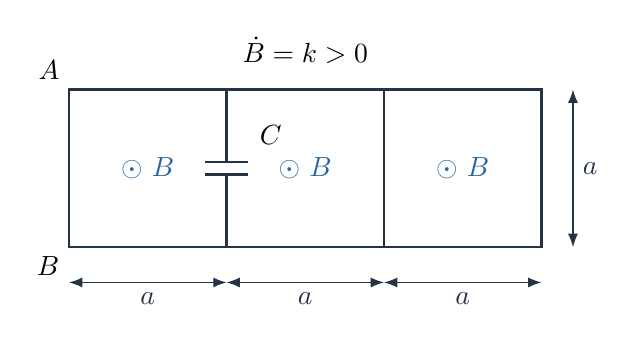
\begin{tikzpicture}
 \network
 \foreach\x in{1,3,5}{\node[blue]at(\x,1){$\odot\ B$};}
 \node[right]at(2.3,1.42){$C$};
 \foreach\x in{0,2,4}{\draw[dim](\x,-.45)--({\x+2},-.45)node[midway,below]{$a$};}
 \draw[dim](6.4,0)--(6.4,2)node[midway,right]{$a$};
 \node at(3,2.5){$\dot B=k>0$};
\end{tikzpicture}
\begin{tikzpicture}
 \network
 \draw[guide](2,.3)--(2,.7)(2,1.3)--(2,1.7);
 \draw[blue,thick,-{Latex}](.8,1)arc[start angle=180,end angle=-130,x radius=1.2,y radius=.55];
 \node[blue]at(1.3,1){$I_1$};
 \draw[green,thick,-{Latex}](4.35,1)arc[start angle=180,end angle=-130,x radius=.65,y radius=.5];
 \node[green]at(5,1){$I_2$};
 \draw[vec](4,1.6)--(4,.45);\node[above]at(4,2.65){$I_1-I_2$};
 \draw[guide](4,2.6)--(4,1.6);
 \draw[vec](0,.5)--(0,1.5);
 \node[above]at(2,2.1){面积 $2a^2$};\node[above]at(5,2.1){面积 $a^2$};
\end{tikzpicture}
\begin{tikzpicture}
 \draw[body](3,3)--(0,3)--(0,0)--(3,0);
 \draw[body](3,0)--(3,1.36)(3,1.64)--(3,3);
 \draw[body](2.55,1.36)--(3.45,1.36)(2.55,1.64)--(3.45,1.64);
 \node[above left]at(0,3){$A$};\node[below left]at(0,0){$B$};
 \node[above right]at(3,3){$P$};\node[below right]at(3,0){$Q$};
 \draw[vec](.5,3)--(2.4,3)node[midway,above]{$I_1$};
 \draw[vec](2.5,0)--(.5,0)node[midway,below]{$I_1$};
 \draw[vec](0,.5)--(0,2.5)node[midway,left]{$I_1$};
 \node[blue]at(1.5,1.5){$\odot\ \dot B>0$};
 \node[red,right]at(3.5,1.85){上极板：$-$};
 \node[red,right]at(3.5,1.1){下极板：$+$};
 \node at(3.2,-.8){$U_C=V_{\rm top}-V_{\rm bottom}<0$};
\end{tikzpicture}
\begin{tikzpicture}
 \network
 \draw[blue,very thick](0,0)--(0,2)--(4,2)(0,0)--(4,0);
 \draw[green,very thick](4,2)--(6,2)--(6,0)--(4,0);
 \draw[red,very thick](4,0)--(4,2);
 \node[blue]at(1,1.5){$I_1$};\node[gray]at(3,1){$i_C=0$};\node[green]at(5,1){$I_2$};
 \draw[red,thick,-{Latex}](4,1.6)--(4,.5);
 \node[red,above]at(4,2.3){$I_1-I_2$};
 \node[blue]at(1.8,-.6){独占五边};\node[green]at(5.2,-.6){独占三边};
\end{tikzpicture}
\end{document}
